%==============================================================
% ICCIT 2026 submission -- IEEE conference format
% FULL VERSION: every section from the original draft is present.
% Exceeds the 6-page ICCIT limit; see "TRIM CANDIDATES" at the bottom.
%
% Format: A4 paper, ANONYMOUS author block, IEEE numeric references.
%
%==============================================================
% STATUS OF THE NUMBERS IN THIS FILE
%
% Reviewer points 1 (threshold leakage) and 2 (duplicate overlap) are both
% RESOLVED; every table and figure has been regenerated from real runs.
%   * AdversarialGen split 300 (adaptation) / 150 (validation) / 200 (sealed
%     test), stratified by label, seed 42.
%   * All 2,650 images screened by pHash, dHash and CLIP cosine; 19 clusters,
%     10 of them straddling partitions; contaminated images removed, leaving
%     148 validation and 194 sealed test images.
%   * Base-split folds rebuilt with StratifiedGroupKFold over those clusters
%     (1,980 groups over 2,000 images), asserted group-disjoint at run time.
%   * tau selected on the clean validation partition only, by a rule fixed
%     before the sweep (argmax fake-class F1, 0.01 grid, ties -> median).
%     -> tau = 0.08 zero-shot, tau = 0.21 domain-adapted.
%   * Clean sealed test scored exactly once at those thresholds.
%   Sources: duplicate_clusters.csv, dedup_summary.txt,
%            adversarialgen_val148_sweep.csv,
%            adversarialgen_leakfree_clean_results.csv,
%            ablation_grouped_summary.csv, baselines_grouped_summary.csv
%
%   * Reviewer point 4 (justify the fusion) is ANSWERED, in the negative:
%     CLIP-only and the fused model are indistinguishable same-distribution on
%     accuracy, AUROC, Brier and ECE, and the fused model is worse calibrated
%     under shift. See Sec. IV-B and fusion_vs_cliponly.csv.
%
%   * Reviewer point 5 (verification) is handled by REMOVAL: the
%     evidence-verification stage is no longer part of this paper's scope.
%     It remains in the implementation. A retrieval measurement we ran on the
%     Bangla corpus (recall@1 0.8%, recall@5 2.5% against gold documents;
%     unrelated Bangla headline pairs sit at median cosine 0.856 versus 0.268
%     for English) is summarised in Sec. V-E as an open problem and is kept in
%     verification_retrieval_summary.txt should you want to report it in full.
%
% STILL OPEN (see the TODO markers):
%   reviewer 6 -- two reference records unverified.
%   reviewer 7 -- still over the 6-page limit.
%
% SELF-CONTAINED BUILD: every figure is drawn in LaTeX (TikZ/pgfplots)
% with its data inline, so this file compiles on its own with no image
% files and no figures/ directory. The image-based variant is
% iccit2026_full.tex.
%
% Before submitting: set \draftnotesfalse (preamble).
%==============================================================
\documentclass[conference,a4paper]{IEEEtran}
\IEEEoverridecommandlockouts

\usepackage{cite}
\usepackage{amsmath,amssymb,amsfonts}
\usepackage{graphicx}
\usepackage{booktabs}
\usepackage{multirow}
\usepackage{graphics}
\usepackage{textcomp}
\usepackage{url}
\usepackage[section]{placeins}
\usepackage{tikz}
\usetikzlibrary{arrows.meta,positioning}
\usepackage{pgfplots}
\pgfplotsset{compat=1.18}

%--------------------------------------------------------------
% FLOAT PLACEMENT. With six figures and four tables, LaTeX's default budget
% (one float per page, 70% of a column) defers most of them and they pile up
% at the end of the document. These settings let a page carry more float and
% less text before it gives up, and [section]{placeins} stops any float
% crossing into the next section.
%--------------------------------------------------------------
\renewcommand{\topfraction}{0.92}
\renewcommand{\bottomfraction}{0.75}
\renewcommand{\textfraction}{0.06}
\renewcommand{\floatpagefraction}{0.65}
\renewcommand{\dbltopfraction}{0.92}
\renewcommand{\dblfloatpagefraction}{0.65}
\setcounter{topnumber}{3}
\setcounter{bottomnumber}{2}
\setcounter{totalnumber}{4}
\setcounter{dbltopnumber}{2}

%--------------------------------------------------------------
% TWO SWITCHES.
%   \blindsubmissiontrue  -> anonymous author block, Acknowledgment hidden
%   \blindsubmissionfalse -> real authors + Acknowledgment printed
%   \draftnotestrue  -> internal "verify before submission" notes PRINT
%   \draftnotesfalse -> those notes are hidden
%
% >>> SET \draftnotesfalse BEFORE YOU SUBMIT. <<<
%--------------------------------------------------------------
\newif\ifblindsubmission
\blindsubmissiontrue      % ICCIT 2026 requires anonymous submission

\newif\ifdraftnotes
\draftnotestrue           % <-- flip to \draftnotesfalse before submitting

\newcommand{\sysname}{SignalCheck}

\begin{document}

%--------------------------------------------------------------
% TITLE -- (A) active, (B) the original draft's title, commented out.
% (B) claims "Feature Fusion" in the title, which Table I does not support.
%--------------------------------------------------------------
\title{\sysname: Multimodal Bangla Fake News Image Detection --
Modality Ablation and Leak-Free Distribution-Shift Evaluation}

% \title{Multimodal Bangla Fake News Detection Through BLIP--CLIP
% Feature Fusion, XGBoost Classification, and Retrieval-Augmented\\
% Dual-LLM Verification}

\ifblindsubmission
  \author{\IEEEauthorblockN{Anonymous Submission}
  \IEEEauthorblockA{Paper ID: XXXX}}
\else
  \author{\IEEEauthorblockN{1\textsuperscript{st} Given Name Surname}
  \IEEEauthorblockA{\textit{dept. name of organization} \\
  \textit{name of organization}\\ City, Country \\ email or ORCID}
  \and
  \IEEEauthorblockN{2\textsuperscript{nd} Given Name Surname}
  \IEEEauthorblockA{\textit{dept. name of organization} \\
  \textit{name of organization}\\ City, Country \\ email or ORCID}
  \and
  \IEEEauthorblockN{3\textsuperscript{rd} Given Name Surname}
  \IEEEauthorblockA{\textit{dept. name of organization} \\
  \textit{name of organization}\\ City, Country \\ email or ORCID}}
\fi

\maketitle

\begin{abstract}
Fake news detection for low-resource languages such as Bangla is held back by
two things: the scarcity of large-scale, image-centric training data, and
classifiers whose reported accuracy comes from evaluation protocols that leak.
This paper presents \sysname, a multimodal classifier for manipulated news
imagery circulating on Bangladeshi social media, together with an evaluation
protocol built to avoid those leaks. The classifier fuses a BLIP-generated
image caption, encoded via multilingual SBERT and refined through Cross-Image
Semantic Fusion (CISF), with a CLIP visual embedding, and classifies the
combined feature vector with a gradient-boosted decision tree. A systematic
per-modality ablation on the BanFakeMM benchmark, evaluated under
duplicate-aware grouped cross-validation, shows that CLIP visual features
dominate classification accuracy, reaching 95.38 percent alone, and that no
text-inclusive configuration differs from it beyond fold-to-fold variation;
OCR, near chance in isolation at 57.35 percent, is removed. We then evaluate
under distribution shift with a protocol designed to be free of selection
effects and of near-duplicate contamination: every partition is screened with
two perceptual hashes and CLIP similarity, the decision threshold is chosen on
a disjoint validation partition, and a sealed test partition is scored exactly
once. Zero-shot transfer to an unseen manipulation style costs 9.8 points of
accuracy and 22.7 points of fake-recall (95.40 to 85.6 percent, 95.70 to
73.0 percent). A validation-selected threshold recovers most of this without
retraining, reaching 91.8 percent accuracy and 95.0 percent fake-recall.
Supervised adaptation on 300 target-style images adds nothing measurable on
top ($+0.0$ points, 95 percent CI $[-3.6, +3.6]$); an earlier draft of this
work reported a gain here, which we retract as an artifact of selecting the
threshold on the evaluation set.
\end{abstract}

%--------------------------------------------------------------
% CCS Concepts -- an ACM block with NO IEEE equivalent, reproduced because it
% was in the original draft. IEEE reviewers will read it as a template
% leftover; consider deleting it.
%--------------------------------------------------------------
\begin{IEEEkeywords}
\textbf{CCS Concepts:} Computing methodologies $\rightarrow$ Machine learning
approaches; Natural language processing; Information systems $\rightarrow$
Multimedia and multimodal retrieval.
\end{IEEEkeywords}

\begin{IEEEkeywords}
Bangla fake news detection, multimodal misinformation, BLIP, CLIP, XGBoost,
distribution shift, domain adaptation, threshold calibration, near-duplicate
leakage, model calibration, low-resource language processing
\end{IEEEkeywords}

%==============================================================
\section{Introduction}
%==============================================================

Bangladesh's social media ecosystem---dominated by Facebook, YouTube, and
messaging-app forwards---has become a primary vector for manipulated and
fabricated news imagery, ranging from digitally altered photocards and forged
documents to fully AI-generated video frames misattributed to public figures.
Unlike text-only misinformation, this class of fake news exploits the combined
visual and textual channel: a viral image is rarely judged on its pixels
alone, but on the claim, caption, or context attached to it as it spreads.

This problem is compounded by linguistic and cultural specificity. Bangla,
unlike English, is a low-resource language for NLP, so most fake-news
detection methods---sentiment, ensemble, graph, and comment-fusion models
alike---have been built and tested only on English datasets from Western
platforms such as LIAR, WELFake and FakeNewsNet. These systems presuppose
signal sources such as dense comment threads or public retweet graphs that are
frequently sparse, unavailable, or structured differently in the Bangladeshi
context. This research identified several core problems in the current state
of Bangla multimodal fake-news detection.

\subsection{Research Problems}

\begin{itemize}
\item \textbf{Training-data scarcity.} No large-scale, organically collected,
labeled dataset of manipulated Bangladeshi news images circulating in
real-world settings exists; training must rely on synthetically constructed
benchmarks such as BanFakeMM.

\item \textbf{Claim-caption divergence.} An uploaded image's automatically
generated caption describes what is visually present in it, not the claim
being asserted about it, so a verdict cannot be reliably reached from the
image alone.

\item \textbf{Same-distribution overstatement.} Same-distribution accuracy is
routinely reported as if it were real-world reliability, without a disjoint
evaluation to check whether a classifier has merely learned one narrow
manipulation style---and, where such an evaluation is reported, the operating
threshold is often tuned on the very set used to report it.
\end{itemize}

\subsection{Approach and Contributions}

\begin{itemize}
\item \textbf{Per-modality ablation.} Deciding which modalities---caption
text, OCR text, CLIP visual features, CISF fusion---actually contribute,
rather than including every available signal by default, and empirically
removing OCR once ablation showed it performs near chance level in isolation.
Results are reported with precision, recall and F1 alongside accuracy.

\item \textbf{Leak-free evaluation under distribution shift.} Partitioning the
shifted split into disjoint adaptation, validation and sealed test subsets;
selecting the decision threshold on validation under a rule fixed in advance;
and scoring the sealed partition exactly once. We separate what is recovered
by thresholding from what is recovered by supervised adaptation, and report
the latter as domain adaptation rather than unseen-style generalization.

\item \textbf{A retracted result.} We report that the training-data
diversification gain claimed in an earlier draft of this work does not survive
a leak-free protocol, and quantify the null result with a confidence interval
and a McNemar test.

\item \textbf{A calibration analysis of the fusion pathway.} Testing whether
the caption channel contributes anything CLIP alone does not, on accuracy,
ranking quality and calibration, in both regimes---and reporting that it does
not.
\end{itemize}

BLIP/CLIP-based multimodal classification is well established, and we do not
claim architectural novelty for it. What we have not found in the Bangla
literature is an image-level manipulation detector evaluated under a protocol
that is simultaneously free of threshold-selection leakage and of
near-duplicate contamination, and that reports what each component actually
contributes. The regional adaptation and the evaluation protocol are where we
locate this work's contribution.

%==============================================================
\section{Literature Review}
%==============================================================

Research on Bangla-language fake news detection remains comparatively limited
relative to English. BanFakeNews \cite{banfakenews} established one of the
earliest large-scale benchmarks for this task: an annotated corpus of roughly
50{,}000 Bangla news items labeled authentic or fabricated, introduced
specifically because most fake-news detection methods have been developed for
English while low-resource languages such as Bangla remain comparatively
under-served. Subsequent work extended this line to multimodal settings.
MultiBanFakeDetect \cite{multibanfake} combines textual and visual fusion
techniques, reporting a hybrid DenseNet-169/mBERT fusion architecture to
detect Bangla fake news in under-resourced contexts, and is, to our knowledge,
the closest prior system to the present work in both language and multimodal
scope. Beyond Bangla specifically, Bansal et al.'s MMCFND framework and its
accompanying MMIFND dataset \cite{mmcfnd} extend multimodal, caption-aware
fake-news detection to seven low-resource Indic languages, including Bengali,
with roughly 28{,}000 labeled instances, and Shibu et al. \cite{banfakenews2}
introduced BanFakeNews-2.0, a 60{,}000-instance manually curated Bangla text
corpus (47{,}000 authentic, 13{,}000 fake).

None of these systems, however, is built around a defined image-manipulation
task with adversarially constructed positive examples---MultiBanFakeDetect
labels whole news articles by their overall claim, and BanFakeNews-2.0 is
text-only---nor does any of them incorporate an external evidence-retrieval or
claim-verification component. Outside the Bangla-specific literature, EANN
\cite{eann}, MVAE \cite{mvae}, and SpotFake \cite{spotfake} each established
that visual and textual signals are complementary for fake-news
classification, but each was developed and validated on English-language,
Western-platform datasets, and none pairs classification with a
retrieval-augmented evidence-verification stage.

A more recent thread of work pairs multimodal classification with
retrieval-augmented, multi-model evidence verification directly. DEFAME
\cite{defame} orchestrates multiple specialized LLM-based experts against
retrieved multimodal evidence; RAGAR \cite{ragar} applies retrieval-augmented
reasoning to political fact-checking with multimodal large language models;
RAMA \cite{rama} proposes a retrieval-augmented multi-agent framework for
multimodal misinformation detection; and CaLM \cite{calm} contrasts a large
and a small language model to verify grounded generation. None of these is
Bangla-specific or Bangladesh-corpus-grounded.

This research identified four critical limitations in the surveyed literature.

\begin{itemize}
\item \textbf{Modality-scope limitation.} Bangla-focused systems are trained
and evaluated on curated news-article datasets rather than the screenshot- and
photocard-style imagery commonly observed circulating on Bangladeshi social
media.

\item \textbf{Verification-scope limitation.} No Bangla-focused system, to our
knowledge, incorporates an external evidence-retrieval or claim-verification
stage alongside image-level classification.

\item \textbf{Generalization-reporting limitation.} General-purpose
retrieval-augmented verification systems such as DEFAME, RAGAR and RAMA are
not Bangla-specific, and Bangla multimodal detectors do not report a disjoint
out-of-distribution evaluation.

\item \textbf{Novelty-attribution limitation.} Prior work sometimes frames
dual-LLM or retrieval-augmented verification as architecturally novel, when
the paradigm itself is already explored in DEFAME, RAGAR, RAMA and CaLM---the
regional adaptation, not the architecture, is where genuine novelty should be
claimed.
\end{itemize}

% NOTE: "genuine out-of-distribution protocol" below is the original wording.
% Sections IV-C and V-B now state that only the zero-shot row measures
% out-of-distribution behaviour, so consider "leak-free distribution-shift
% protocol" here for consistency. Left as written pending your decision.
This paper addresses the first and third of these limitations: it targets
image-level manipulation detection on screenshot/photocard-style imagery (via
BanFakeMM) and evaluates that classifier under a leak-free distribution-shift
protocol. The verification-scope limitation is not addressed here; an
evidence-retrieval stage exists in the implementation but is outside this
paper's evaluated scope, and we make no claim about it.

%==============================================================
\section{Methodology}
%==============================================================

\subsection{System Architecture}

\sysname{} is a local multimodal classifier that assigns a fake-probability
score to an uploaded image using only its visual and captioned content. Three
representations are extracted per image---a BLIP caption encoded by
multilingual SBERT and refined through Cross-Image Semantic Fusion, a CLIP
visual embedding, and TF-IDF features over the processed caption---and the
concatenated vector is classified by a gradient-boosted decision tree.
Fig.~\ref{fig:arch} illustrates the pipeline.

\emph{Scope.} This paper reports the classifier only. A retrieval-augmented
evidence-verification stage exists in the implementation but is not evaluated
here and no claim in this paper depends on it; Section~\ref{sec:limitations}
states what its evaluation would require.

\begin{figure*}[!t]
\centering
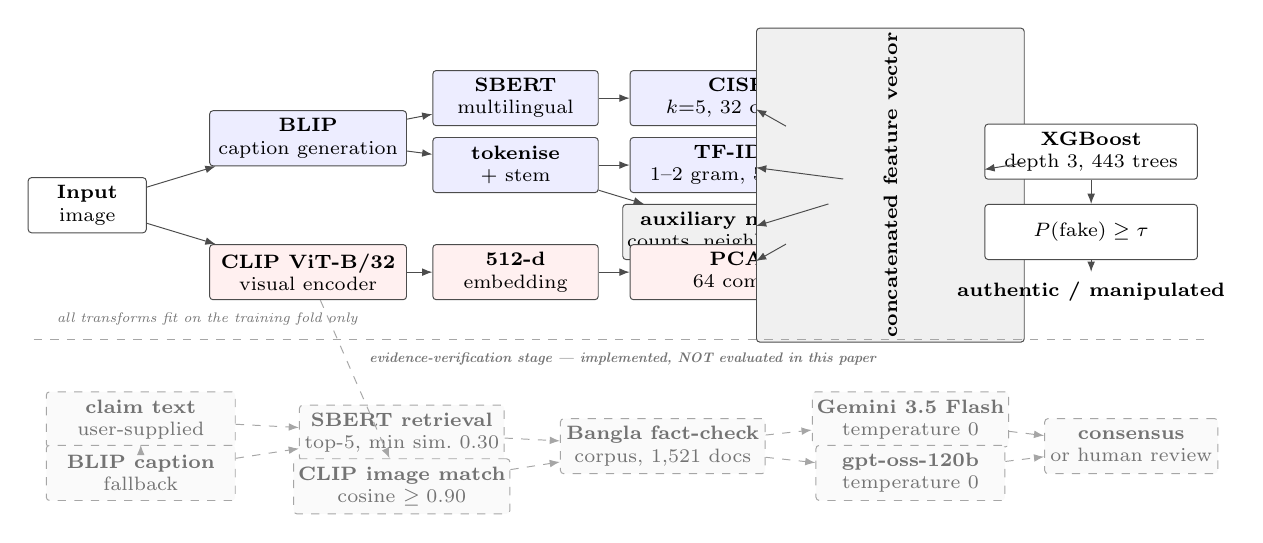
\begin{tikzpicture}[
  x=0.85mm, y=0.85mm, font=\scriptsize,
  blk/.style   = {draw=black!70, rounded corners=1.2pt, line width=0.35pt,
                  align=center, inner sep=1.6pt, minimum height=7mm},
  txtp/.style  = {blk, fill=blue!7},
  visp/.style  = {blk, fill=red!6},
  shrd/.style  = {blk, fill=black!6},
  plain/.style = {blk, fill=white},
  ghost/.style = {blk, dashed, draw=black!35, fill=black!2, text=black!55},
  ar/.style    = {-{Latex[length=1.3mm]}, draw=black!70, line width=0.35pt},
  gar/.style   = {-{Latex[length=1.3mm]}, draw=black!35, line width=0.35pt, dashed},
]
% ---------- evaluated band ----------
\node[plain, minimum width=15mm] (img)   at (8,  42) {\textbf{Input}\\image};
\node[txtp, minimum width=25mm]  (blip)  at (41, 52) {\textbf{BLIP}\\caption generation};
\node[visp, minimum width=25mm]  (clip)  at (41, 32) {\textbf{CLIP ViT-B/32}\\visual encoder};
\draw[ar] (img) -- (blip);   \draw[ar] (img) -- (clip);

\node[txtp, minimum width=21mm] (sbert) at (72, 58) {\textbf{SBERT}\\multilingual};
\node[txtp, minimum width=21mm] (tok)   at (72, 48) {\textbf{tokenise}\\+ stem};
\node[visp, minimum width=21mm] (d512)  at (72, 32) {\textbf{512-d}\\embedding};
\draw[ar] (blip) -- (sbert); \draw[ar] (blip) -- (tok); \draw[ar] (clip) -- (d512);

\node[txtp, minimum width=27mm] (cisf)  at (105, 58) {\textbf{CISF}\\$k{=}5$, 32 comp.};
\node[txtp, minimum width=27mm] (tfidf) at (105, 48) {\textbf{TF-IDF}\\1--2 gram, 5{,}000-d};
\node[shrd, minimum width=27mm] (num)   at (105, 38) {\textbf{auxiliary numeric}\\counts, neighbour sim.};
\node[visp, minimum width=27mm] (pca)   at (105, 32) {\textbf{PCA}\\64 comp.};
\draw[ar] (sbert) -- (cisf); \draw[ar] (tok) -- (tfidf);
\draw[ar] (tok) -- (num);    \draw[ar] (d512) -- (pca);

\node[shrd, minimum width=5mm, minimum height=34mm, rotate=90]
     (cat) at (128, 45) {\textbf{concatenated feature vector}};
\foreach \s in {cisf, tfidf, num, pca} { \draw[ar] (\s) -- (cat); }

\node[plain, minimum width=27mm] (xgb) at (158, 50) {\textbf{XGBoost}\\depth 3, 443 trees};
\node[plain, minimum width=27mm] (thr) at (158, 38) {$P(\mathrm{fake}) \geq \tau$};
\draw[ar] (cat) -- (xgb); \draw[ar] (xgb) -- (thr);
\node[below=1.5mm of thr, font=\scriptsize\bfseries] (out) {authentic / manipulated};
\draw[ar] (thr) -- (out);
\node[anchor=west, font=\tiny\itshape, text=black!55] at (2, 25)
     {all transforms fit on the training fold only};

% ---------- out-of-scope band ----------
\draw[dashed, draw=black!35, line width=0.35pt] (0, 22) -- (176, 22);
\node[font=\tiny\bfseries\itshape, text=black!55] at (88, 19)
     {evidence-verification stage --- implemented, NOT evaluated in this paper};

\node[ghost, minimum width=24mm] (claim) at (16,  10) {\textbf{claim text}\\user-supplied};
\node[ghost, minimum width=24mm] (capfb) at (16,   2) {\textbf{BLIP caption}\\fallback};
\node[ghost, minimum width=26mm] (ret)   at (55,   8) {\textbf{SBERT retrieval}\\top-5, min sim.\ 0.30};
\node[ghost, minimum width=26mm] (imatch)at (55,   0) {\textbf{CLIP image match}\\cosine $\geq 0.90$};
\node[ghost, minimum width=26mm] (corp)  at (94,   6) {\textbf{Bangla fact-check}\\corpus, 1{,}521 docs};
\node[ghost, minimum width=24mm] (gem)   at (131, 10) {\textbf{Gemini 3.5 Flash}\\temperature 0};
\node[ghost, minimum width=24mm] (oss)   at (131,  2) {\textbf{gpt-oss-120b}\\temperature 0};
\node[ghost, minimum width=22mm] (cons)  at (164,  6) {\textbf{consensus}\\or human review};
\draw[gar] (claim) -- (capfb);
\draw[gar] (claim) -- (ret);   \draw[gar] (capfb) -- (ret);
\draw[gar] (clip)  -- (imatch);
\draw[gar] (ret)   -- (corp);  \draw[gar] (imatch) -- (corp);
\draw[gar] (corp)  -- (gem);   \draw[gar] (corp)  -- (oss);
\draw[gar] (gem)   -- (cons);  \draw[gar] (oss)   -- (cons);
\end{tikzpicture}
\caption{\sysname{} architecture. \textbf{Upper band (evaluated):} four
feature blocks are concatenated---the CISF-refined caption embedding, a TF-IDF
representation of the same caption, auxiliary numeric features (token counts
and CISF neighbour-similarity statistics), and the reduced CLIP visual
embedding---and classified by a gradient-boosted tree. OCR is absent by design
(Section~\ref{sec:ablation}). \textbf{Lower band (dashed, not evaluated):} the
evidence-verification stage present in the implementation. It reuses the same
CLIP embedding for direct image matching. No result in this paper depends on
it and we make no claim about its accuracy; see
Section~\ref{sec:limitations}.}
\label{fig:arch}
\end{figure*}

\subsection{Dataset and Partitioning}
\label{sec:data}

The classifier is trained and evaluated on the AdversarialEdit split of the
public BanFakeMM benchmark \cite{banfakemm}: 2{,}000 images, 1{,}000 authentic
and 1{,}000 manipulated, giving a class-balanced base dataset. BanFakeMM
constructs its ``fake'' images through a defined editing or generation
pipeline rather than through subjective human annotation of ambiguous
real-world content, so ground-truth labels are deterministic by construction.

Behaviour under distribution shift is measured on BanFakeMM's AdversarialGen
split (2{,}000 fully AI-generated images), which is divided into three
mutually disjoint subsets:

\begin{itemize}
\item \textbf{300 images} used only for the supervised adaptation experiment
of Section~\ref{sec:shift};
\item \textbf{150 images} (75 authentic, 75 manipulated) used only for
decision-threshold selection;
\item \textbf{200 images} (100 authentic, 100 manipulated) sealed as the final
test partition, used in no training, tuning, or threshold-selection step and
scored exactly once.
\end{itemize}

Assignment is stratified by label with a fixed seed (42). The remaining
1{,}500 AdversarialGen images are unused. Section~\ref{sec:dedup} then screens
these partitions for near-duplicates and removes the contaminated images,
leaving 148 validation and 194 test images.

\subsubsection{Near-duplicate screening}
\label{sec:dedup}
Filename comparison is not sufficient here: a manipulated image is an edited
copy of an authentic one, so the two can carry unrelated names and still be
the same picture. Every one of the 2{,}650 images the study actually uses
(2{,}000 base split plus the 650 AdversarialGen images above) is therefore
screened by content. Each image is reduced to a 64-bit DCT perceptual hash
(pHash), a 64-bit difference hash (dHash), and its CLIP embedding; a pair is
treated as a near-duplicate when the pHash or dHash Hamming distance is at
most 2 or the CLIP cosine similarity is at least 0.98, and pairs are merged
into clusters with union-find.

These thresholds sit in a clear gap rather than being chosen arbitrarily. Of
the 3.5 million candidate pairs, 94 lie at pHash distance 0 and only 102 at
distance 6 or below; 93 lie at cosine 0.999 or above and 117 at 0.95 or above.
Duplicates are near-exact, and any looser setting begins chaining unrelated
images into implausible clusters through transitive merges.

The screen links 118 pairs into 19 multi-image clusters covering 58 images.
Ten of those clusters span more than one partition: 6 of the 200 sealed test
images (3.0 percent), 2 of the 150 validation images (1.3 percent) and 11 of
the 300 adaptation images (3.7 percent) have a near-duplicate inside the base
training set. All contaminated images are removed, leaving a 194-image sealed
test partition (100 manipulated, 94 authentic) and a 148-image validation
partition. Within the base split itself, the screen yields 1{,}980 groups over
2{,}000 images, and every cross-validation fold in Section~\ref{sec:ablation}
is built with \texttt{StratifiedGroupKFold} over those groups, so an image and
all of its near-duplicates always fall on the same side of a split. Fold
assignments are asserted group-disjoint at run time.

\emph{Remaining caveat.} One criterion we tested and discarded is worth
recording: we initially also merged images sharing a filename stem across the
real and fake folders, on the assumption that a shared numeric id marks an
original and its edit. Calibrating that assumption against the 38 such stems
in the base split showed those pairs are statistically indistinguishable from
random pairs (pHash distance median 32 versus 32, CLIP cosine 0.51 versus
0.40). In BanFakeMM a shared id does not indicate a source relationship, so
the criterion was removed. Source-article provenance is not published with the
benchmark and therefore cannot be grouped on directly; the content-based
screen is our proxy for it.

\subsubsection{Preprocessing steps}

\begin{itemize}
\item \textbf{Captioning and OCR.} A BLIP model generates a natural-language
caption describing each image's visual content. OCR-based text extraction was
evaluated during an earlier ablation phase and found to perform near the
chance level in isolation on this dataset (57.35 percent accuracy); since the
final CLIP-based configuration achieved comparable accuracy without it, OCR
was excluded from the final preprocessing pipeline.

\item \textbf{Text processing and embedding.} The caption is tokenized and
stemmed, with separate handling for English and Bangla script, to produce a
processed-text representation used for TF-IDF features, and separately encoded
into a dense semantic embedding via a multilingual SBERT model.

\item \textbf{Visual embedding.} A CLIP vision encoder independently extracts
a 512-dimensional visual embedding directly from the image pixels.
\end{itemize}

\subsection{Multimodal Feature Fusion and Classification}

For each input image, three complementary representations are extracted. The
BLIP caption is encoded into a semantic embedding using SBERT, then refined
through Cross-Image Semantic Fusion (CISF): the embedding is combined with the
weighted average of its $k=5$ nearest semantic neighbours within the training
corpus, using a fusion weight of $\alpha=0.65$ favouring the original
embedding, and the fused vector is re-normalized and reduced to 32 principal
components via PCA. In parallel, the CLIP visual embedding (512-dimensional)
is separately reduced to 64 principal components via its own PCA transform,
fit only on the training fold in the same way as the caption pathway's
reduction---this keeps the two embedding blocks on a comparable scale relative
to the lower-dimensional TF-IDF and numeric features.

The neighbour count ($k=5$), fusion weight ($\alpha=0.65$), and target
dimensionality (32 components) were fixed design choices for this study rather
than selected through a dedicated validation search; a systematic sensitivity
study over these hyperparameters, and comparison against adaptive fusion
mechanisms such as MMFusionNet \cite{mmfusionnet} or CLAAF \cite{claaf}, is
left for future work. To prevent leakage, each training embedding's own
nearest-neighbour search excludes itself when the fusion reference set is
constructed, and at inference time an unseen image's embedding is compared
only against this fixed, pre-established training-set reference.

The final feature vector concatenates four blocks, each fit only on the
training fold: the 32-component CISF-fused caption embedding, the 64-component
CLIP embedding, a TF-IDF representation over the processed caption text
(unigrams and bigrams, vocabulary capped at 5{,}000 features, minimum document
frequency 3), and a small set of auxiliary numeric features (token counts,
neighbour-similarity statistics). This combined representation is passed to a
gradient-boosted decision tree classifier (XGBoost).

\subsection{Training Configuration and Threshold Selection}
\label{sec:training}

XGBoost hyperparameters were selected via randomized search (scikit-learn's
\texttt{RandomizedSearchCV}, 8 sampled configurations under 3-fold
cross-validation, scored by fake-class F1)---a comparatively small search
budget chosen for computational cost. The selected configuration is
\texttt{max\_depth}~3, \texttt{learning\_rate}~0.0742,
\texttt{n\_estimators}~443, \texttt{subsample}~0.866,
\texttt{colsample\_bytree}~0.683, \texttt{min\_child\_weight}~2,
\texttt{gamma}~0.143, \texttt{reg\_alpha}~$1.01\times10^{-5}$ and
\texttt{reg\_lambda}~4.911.

The classifier outputs a fake-probability score in $[0,1]$. The operating
threshold is selected on held-out validation data and never on the evaluation
partition. The selection rule was fixed before the sweep was run: $\tau$ is
the threshold maximizing fake-class F1 on the screened 148-image validation
partition over a $0.01$-step grid, with ties broken by the median of the tied
run. This yields $\tau = 0.08$ for the zero-shot model and $\tau = 0.21$ for
the domain-adapted model (Fig.~\ref{fig:sweep}). The sealed 194-image test
partition is then scored exactly once at the corresponding threshold, after
all training and threshold decisions are frozen, and is used for no tuning of
any kind.

Per-modality ablation results (Section~\ref{sec:ablation}) come from repeated
stratified 5-fold \emph{grouped} cross-validation over the near-duplicate
clusters of Section~\ref{sec:dedup} (2 repeats per configuration, 10 folds
total), with identical fold splits and fixed hyperparameters held constant
across every evaluated feature configuration. All dimensionality-reduction
transforms, vocabularies and neighbour reference sets are fit inside the
training fold only. Every same-distribution figure in
Section~\ref{sec:ablation} is computed at the conventional $\tau = 0.50$
cut-off, not at a tuned threshold: no threshold search is performed on the
base split at all, so those numbers carry no selection effect. Threshold
selection is confined to the distribution-shift experiment, where the
asymmetric cost of a missed manipulation makes the operating point a real
design decision.

\emph{Reproducibility.} Fold assignment, the randomized search, the PCA
transforms and the classifier all use a fixed random seed of 42. Software
versions, exact BLIP/CLIP/SBERT checkpoint identifiers, hardware and
end-to-end runtime are given in the supplementary material; the partition
manifests, per-image probabilities, the full validation sweep and the sealed
test results are released alongside the code.

\subsection{Evaluation Metrics}

Classification results are reported as accuracy, precision, recall and F1 for
the manipulated class, with real-class recall additionally reported under
distribution shift, since accuracy alone can mask asymmetric degradation
between classes. Fake-recall is treated as the more safety-critical metric,
since a missed manipulated image can circulate unchecked whereas a false alarm
on an authentic image costs only a review step; this asymmetric cost is why
the selection rule of Section~\ref{sec:training} maximizes fake-class F1.
Accuracy on the sealed test partition is accompanied by a bootstrap 95 percent
confidence interval (5{,}000 resamples), and the adaptation contrast is tested
with McNemar's test on discordant predictions.

%==============================================================
\section{Experimental Results}
%==============================================================

\subsection{Classifier Ablation Performance}
\label{sec:ablation}

\begin{table}[!tb]
\caption{Per-Modality Ablation on the Base Split, Repeated Stratified 5-Fold
\emph{Grouped} Cross-Validation Over Near-Duplicate Clusters ($2$ Repeats,
$10$ Folds). Accuracy Shown as Mean $\pm$ Standard Deviation Across Folds.
All Values in Percent.}
\label{tab:ablation}
\centering
\setlength{\tabcolsep}{3.5pt}
\begin{tabular}{lcccc}
\toprule
\textbf{Configuration} & \textbf{Acc.} & \textbf{Prec.$_{f}$} &
\textbf{Rec.$_{f}$} & \textbf{F1$_{f}$} \\
\midrule
OCR only              & 57.35 $\pm$ 2.34 & 63.97 & 33.85 & 44.22 \\
Caption only          & 74.50 $\pm$ 2.68 & 75.22 & 73.25 & 74.16 \\
Text only             & 76.05 $\pm$ 1.82 & 76.42 & 75.45 & 75.87 \\
Text + CISF           & 77.38 $\pm$ 2.10 & 77.41 & 77.55 & 77.40 \\
\midrule
CLIP only             & 95.38 $\pm$ 1.33 & 94.68 & 96.15 & 95.41 \\
Text + CLIP           & 95.28 $\pm$ 1.04 & 95.04 & 95.55 & 95.28 \\
CLIP + CISF           & 95.23 $\pm$ 1.38 & 95.07 & 95.40 & 95.23 \\
Caption + CISF + CLIP & \textbf{95.40} $\pm$ 1.09 & 95.13 & 95.70 & 95.41 \\
\bottomrule
\multicolumn{5}{l}{\footnotesize Subscript $f$ denotes the manipulated
(``fake'') class.}
\end{tabular}
\end{table}

\begin{figure}[!tb]
\centering
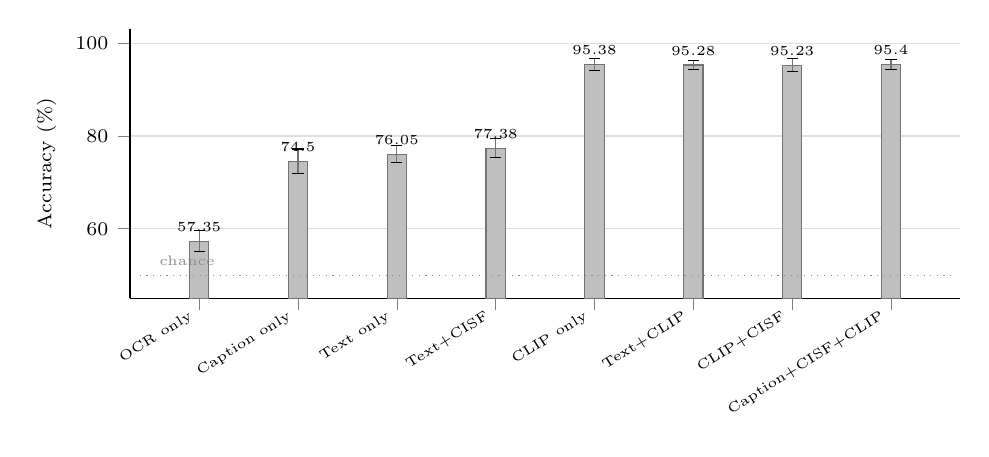
\begin{tikzpicture}
\begin{axis}[
  width=\columnwidth, height=5.0cm, font=\scriptsize,
  ybar, bar width=7pt, ymin=45, ymax=103,
  ylabel={Accuracy (\%)}, ylabel near ticks,
  xtick={0,1,2,3,4,5,6,7}, xticklabels={{OCR only},{Caption only},{Text only},{Text+CISF},{CLIP only},{Text+CLIP},{CLIP+CISF},{Caption+CISF+CLIP}},
  xticklabel style={rotate=32, anchor=east, font=\tiny},
  ymajorgrids, grid style={black!12},
  axis lines*=left, tick align=outside,
  nodes near coords, nodes near coords style={font=\tiny, /pgf/number format/fixed,
    /pgf/number format/precision=2},
  error bars/y dir=both, error bars/y explicit,
]
\addplot[fill=black!25, draw=black!55] table[x index=0, y index=1,
  y error index=2] {
0 57.35 2.34
1 74.50 2.68
2 76.05 1.82
3 77.38 2.10
4 95.38 1.33
5 95.28 1.04
6 95.23 1.38
7 95.40 1.09
};
\draw[dotted, black!45] (axis cs:-0.6,50) -- (axis cs:7.6,50);
\node[font=\tiny, text=black!45, anchor=south west] at (axis cs:-0.5,50)
  {chance};
\end{axis}
\end{tikzpicture}
\caption{Per-modality ablation accuracy (repeated stratified 5-fold grouped
cross-validation; error bars are one standard deviation across folds).}
\label{fig:ablation}
\end{figure}

Table~\ref{tab:ablation} and Fig.~\ref{fig:ablation} report every feature
configuration under an identical protocol. Three results matter.

First, OCR text in isolation reaches 57.35 percent accuracy, close to the
50 percent chance baseline for this balanced binary task, with fake-recall of
only 33.85 percent. This is the empirical basis for removing OCR. We do not
generalize this beyond BanFakeMM: MultiBanFakeDetect \cite{multibanfake}
indicates that text-in-image remains a meaningful vector for Bangla
misinformation more broadly, and BanFakeMM's manipulations are photographic
rather than text-embedded.

Second, all text-only configurations saturate below 78 percent, while any
configuration containing CLIP exceeds 95 percent. Visual features, not caption
text or its derived properties, carry the discriminative signal for this task.

Third---and this is a negative result we report rather than obscure---no
CLIP-containing configuration is distinguishable from any other. CLIP-only
reaches 95.38 $\pm$ 1.33 percent, adding CISF on top gives
95.23 $\pm$ 1.38, and the full caption+CISF+CLIP configuration gives
95.40 $\pm$ 1.09. The entire spread across these four configurations is
0.17 points against a per-fold standard deviation of 1.0--1.4 points.

The ordering here is itself instructive. Under the ungrouped folds used in an
earlier version of this analysis, CLIP-only led the fused configuration by
0.18 points; under duplicate-aware folds the fused configuration leads by
0.02. Both gaps are far inside one fold's variation, and the fact that the
ranking reverses when an unrelated methodological change is made is the
clearest evidence that the ranking was never resolvable in the first place. We
therefore do not read the new ordering as support for the fusion pathway.

\subsection{Does the Caption Pathway Contribute?}
\label{sec:fusion}

Accuracy parity alone does not settle whether the caption pathway is worth
keeping: a feature block can leave accuracy unchanged and still improve how
well the scores rank examples, or how well the predicted probabilities are
calibrated. Both are exactly the properties a deployed screening system needs,
and neither is visible in Table~\ref{tab:ablation}. We therefore compare
CLIP-only against the full fused configuration on four measures, in both
regimes, with everything else held fixed.

\begin{table}[!tb]
\caption{CLIP-Only Versus the Fused Configuration, Same Hyperparameters and
Folds. AUROC and Brier Are Threshold-Independent; ECE Is Expected Calibration
Error Over $10$ Bins. Arrows Mark the Preferred Direction.}
\label{tab:fusion}
\centering
\setlength{\tabcolsep}{4pt}
\begin{tabular}{llcccc}
\toprule
& \textbf{Model} & \textbf{Acc.}$\uparrow$ & \textbf{AUROC}$\uparrow$ &
\textbf{Brier}$\downarrow$ & \textbf{ECE}$\downarrow$ \\
\midrule
\multirow{2}{*}{\rotatebox{90}{\scriptsize same-d.}}
& CLIP only & 95.38 & 0.9918 & 0.0349 & 3.17 \\
& Fused     & 95.40 & 0.9920 & 0.0342 & 3.05 \\
\midrule
\multirow{2}{*}{\rotatebox{90}{\scriptsize shift}}
& CLIP only & 85.05 & \textbf{0.9759} & \textbf{0.0936} & \textbf{4.06} \\
& Fused     & 85.57 & 0.9732 & 0.1076 & 7.31 \\
\bottomrule
\multicolumn{6}{p{0.94\columnwidth}}{\footnotesize Same-distribution figures
are pooled out-of-fold values over the grouped folds of
Table~\ref{tab:ablation}; shift figures are the screened 194-image sealed
partition at the default $\tau = 0.50$, so the two models are compared at the
same operating point.}
\end{tabular}
\end{table}

Table~\ref{tab:fusion} gives the result. Same-distribution, the two models are
indistinguishable on every measure. Across the ten grouped folds the paired
differences (fused minus CLIP-only) are $+0.03$ accuracy points
(95\% CI $[-0.43, +0.45]$, Wilcoxon $p = 1.000$), $+0.0002$ AUROC
($[-0.0007, +0.0011]$, $p = 0.432$), $-0.0006$ Brier
($[-0.0021, +0.0012]$, $p = 0.232$) and $-0.12$ ECE points
($[-0.60, +0.31]$, $p = 0.695$). McNemar on the pooled out-of-fold predictions
finds 21 images the fused model alone gets right against 20 for CLIP-only.
Every interval spans zero.

Under distribution shift the comparison stops being neutral and turns against
the caption pathway. The fused model's accuracy advantage, $+0.5$ points, is
well inside its confidence interval ($[-2.6, +3.6]$), but its ranking is
slightly worse (AUROC $0.9732$ against $0.9759$) and its calibration is
clearly worse: Brier rises from $0.0936$ to $0.1076$ and expected calibration
error from $4.06$ to $7.31$ percentage points. The caption pathway does not
merely fail to help under shift; it makes the probability estimates less
trustworthy at the moment they matter most, which is precisely when the
operating threshold has to be chosen.

\emph{We therefore do not claim the fusion as a contribution.} The caption
pathway was included on the reasonable prior that a semantic channel would
complement a visual one, and this study's own evidence does not support that
prior on this task: it costs a BLIP forward pass, an SBERT encoding and a
nearest-neighbour search per image, and returns nothing measurable
same-distribution and a calibration penalty under shift. A practitioner
building on this work should use CLIP features with a gradient-boosted tree
and stop there. We report the fused configuration as the system we built and
evaluated, with this negative result attached, rather than quietly presenting
the simpler model as though it had been the plan all along.

\subsection{Final Configuration Evaluation}

The selected final configuration---caption text fused via CISF, combined with
CLIP features, without OCR---reaches 95.40 $\pm$ 1.09 percent
same-distribution accuracy, with fake-class precision 95.13 percent, recall
95.70 percent and F1 95.41 percent. These are cross-validated means rather
than a single held-out confusion matrix, since the base-split protocol
(Section~\ref{sec:training}) uses repeated $k$-fold grouped cross-validation
rather than one fixed train/test split; per-fold true and false-positive counts were
not separately retained, so a single confusion matrix for the base split is
not reported here.

\subsection{Performance Under Distribution Shift}
\label{sec:shift}

\begin{table}[!tb]
\caption{Evaluation Under Distribution Shift. Thresholds Were Selected on a
Disjoint 148-Image Validation Partition; the Sealed 194-Image Test Partition
Was Scored Exactly Once. Both Partitions Are Near-Duplicate Screened
(Section~\ref{sec:dedup}). All Values in Percent.}
\label{tab:shift}
\centering
\setlength{\tabcolsep}{3pt}
\begin{tabular}{llccccc}
\toprule
\textbf{Setting} & \textbf{$\tau$} & \textbf{Acc.} & \textbf{Prec.$_{f}$} &
\textbf{Rec.$_{f}$} & \textbf{Rec.$_{r}$} & \textbf{F1$_{f}$} \\
\midrule
\multicolumn{7}{l}{\emph{Zero-shot transfer (no target-style data in training)}} \\
Default threshold   & 0.50 & 85.6 & 98.6 & 73.0 & 98.9 & 83.9 \\
Validation-selected & 0.08 & \textbf{91.8} & 89.6 & 95.0 & 88.3 & 92.2 \\
\midrule
\multicolumn{7}{l}{\emph{Supervised domain adaptation ($+300$ AdversarialGen images)}} \\
Validation-selected & 0.21 & \textbf{91.8} & 90.4 & 94.0 & 89.4 & 92.2 \\
\bottomrule
\multicolumn{7}{p{0.95\columnwidth}}{\footnotesize Bootstrap 95\% confidence
intervals on accuracy (5{,}000 resamples): $[80.4, 90.2]$, $[87.6, 95.4]$ and
$[87.6, 95.4]$ respectively. Subscripts $f$ and $r$ denote the manipulated and
authentic classes.}
\end{tabular}
\end{table}

\begin{figure}[!tb]
\centering
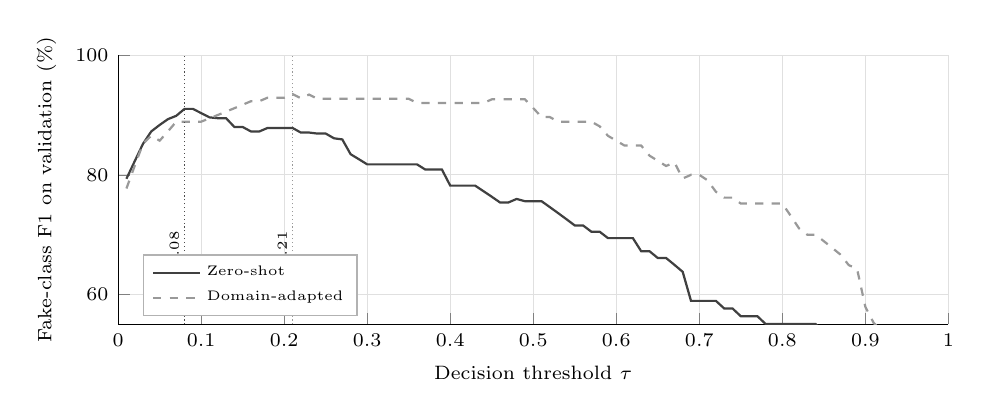
\begin{tikzpicture}
\begin{axis}[
  width=\columnwidth, height=5.0cm, font=\scriptsize,
  xlabel={Decision threshold $\tau$},
  ylabel={Fake-class F1 on validation (\%)},
  xmin=0, xmax=1, ymin=55, ymax=100,
  ymajorgrids, xmajorgrids, grid style={black!12},
  axis lines*=left, legend pos=south west,
  legend style={font=\tiny, draw=black!30}, legend cell align=left,
]
\addplot[black!75, thick, mark=none] coordinates {
(0.01,79.35)
(0.02,82.29)
(0.03,85.21)
(0.04,87.27)
(0.05,88.34)
(0.06,89.31)
(0.07,89.87)
(0.08,91.03)
(0.09,91.03)
(0.10,90.32)
(0.11,89.61)
(0.12,89.47)
(0.13,89.47)
(0.14,88.00)
(0.15,88.00)
(0.16,87.25)
(0.17,87.25)
(0.18,87.84)
(0.19,87.84)
(0.20,87.84)
(0.21,87.84)
(0.22,87.07)
(0.23,87.07)
(0.24,86.90)
(0.25,86.90)
(0.26,86.11)
(0.27,85.92)
(0.28,83.45)
(0.29,82.61)
(0.30,81.75)
(0.31,81.75)
(0.32,81.75)
(0.33,81.75)
(0.34,81.75)
(0.35,81.75)
(0.36,81.75)
(0.37,80.88)
(0.38,80.88)
(0.39,80.88)
(0.40,78.20)
(0.41,78.20)
(0.42,78.20)
(0.43,78.20)
(0.44,77.27)
(0.45,76.34)
(0.46,75.38)
(0.47,75.38)
(0.48,75.97)
(0.49,75.59)
(0.50,75.59)
(0.51,75.59)
(0.52,74.60)
(0.53,73.60)
(0.54,72.58)
(0.55,71.54)
(0.56,71.54)
(0.57,70.49)
(0.58,70.49)
(0.59,69.42)
(0.60,69.42)
(0.61,69.42)
(0.62,69.42)
(0.63,67.23)
(0.64,67.23)
(0.65,66.10)
(0.66,66.10)
(0.67,64.96)
(0.68,63.79)
(0.69,58.93)
(0.70,58.93)
(0.71,58.93)
(0.72,58.93)
(0.73,57.66)
(0.74,57.66)
(0.75,56.36)
(0.76,56.36)
(0.77,56.36)
(0.78,55.05)
(0.79,55.05)
(0.80,55.05)
(0.81,55.05)
(0.82,55.05)
(0.83,55.05)
(0.84,55.05)
(0.85,53.70)
(0.86,52.34)
(0.87,50.94)
(0.88,50.94)
(0.89,48.08)
(0.90,46.60)
(0.91,42.00)
(0.92,37.50)
(0.93,28.57)
(0.94,28.57)
(0.95,26.67)
(0.96,25.00)
(0.97,14.63)
(0.98,10.13)
(0.99,5.19)
};
\addlegendentry{Zero-shot}
\addplot[black!40, thick, dashed, mark=none] coordinates {
(0.01,77.72)
(0.02,81.52)
(0.03,85.23)
(0.04,86.55)
(0.05,85.71)
(0.06,87.27)
(0.07,88.89)
(0.08,88.89)
(0.09,88.89)
(0.10,88.89)
(0.11,89.44)
(0.12,90.00)
(0.13,90.57)
(0.14,91.14)
(0.15,91.72)
(0.16,92.31)
(0.17,92.31)
(0.18,92.90)
(0.19,92.90)
(0.20,92.90)
(0.21,93.51)
(0.22,92.81)
(0.23,93.42)
(0.24,92.72)
(0.25,92.72)
(0.26,92.72)
(0.27,92.72)
(0.28,92.72)
(0.29,92.72)
(0.30,92.72)
(0.31,92.72)
(0.32,92.72)
(0.33,92.72)
(0.34,92.72)
(0.35,92.72)
(0.36,92.00)
(0.37,92.00)
(0.38,92.00)
(0.39,92.00)
(0.40,92.00)
(0.41,92.00)
(0.42,92.00)
(0.43,92.00)
(0.44,92.00)
(0.45,92.62)
(0.46,92.62)
(0.47,92.62)
(0.48,92.62)
(0.49,92.62)
(0.50,91.16)
(0.51,89.66)
(0.52,89.66)
(0.53,88.89)
(0.54,88.89)
(0.55,88.89)
(0.56,88.89)
(0.57,88.89)
(0.58,88.11)
(0.59,86.52)
(0.60,85.71)
(0.61,84.89)
(0.62,84.89)
(0.63,84.89)
(0.64,83.21)
(0.65,82.35)
(0.66,81.48)
(0.67,82.09)
(0.68,79.39)
(0.69,80.00)
(0.70,80.00)
(0.71,79.07)
(0.72,77.17)
(0.73,76.19)
(0.74,76.19)
(0.75,75.20)
(0.76,75.20)
(0.77,75.20)
(0.78,75.20)
(0.79,75.20)
(0.80,75.20)
(0.81,73.17)
(0.82,71.07)
(0.83,70.00)
(0.84,70.00)
(0.85,68.91)
(0.86,67.80)
(0.87,66.67)
(0.88,64.91)
(0.89,64.29)
(0.90,57.94)
(0.91,55.24)
(0.92,53.85)
(0.93,52.43)
(0.94,49.50)
(0.95,44.90)
(0.96,35.16)
(0.97,31.46)
(0.98,23.53)
(0.99,17.07)
};
\addlegendentry{Domain-adapted}
\draw[densely dotted, black!70] (axis cs:0.08,55) -- (axis cs:0.08,100);
\draw[densely dotted, black!40] (axis cs:0.21,55) -- (axis cs:0.21,100);
\node[font=\tiny, anchor=south west, rotate=90] at (axis cs:0.085,57)
  {$\tau^{*}{=}0.08$};
\node[font=\tiny, anchor=south west, rotate=90] at (axis cs:0.215,57)
  {$\tau^{*}{=}0.21$};
\end{axis}
\end{tikzpicture}
\caption{Fake-class F1 against decision threshold on the 148-image validation
partition. $\tau^{*}$ is the argmax under the rule fixed in
Section~\ref{sec:training}; the sealed test partition plays no part in this
selection.}
\label{fig:sweep}
\end{figure}

\begin{figure}[!tb]
\centering
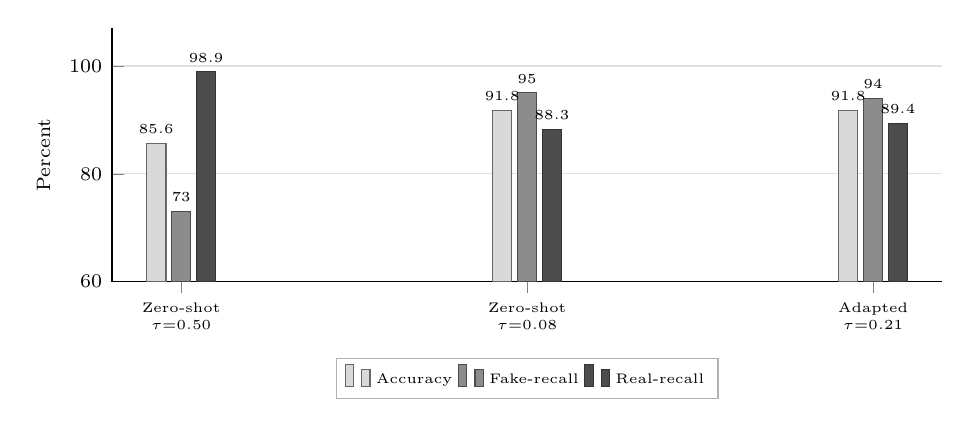
\begin{tikzpicture}
\begin{axis}[
  width=\columnwidth, height=4.8cm, font=\scriptsize,
  ybar, bar width=7pt, ymin=60, ymax=107,
  ylabel={Percent}, ylabel near ticks,
  xtick={0,1,2}, xticklabels={{Zero-shot\\$\tau{=}0.50$},{Zero-shot\\$\tau{=}0.08$},{Adapted\\$\tau{=}0.21$}},
  xticklabel style={font=\tiny, align=center},
  ymajorgrids, grid style={black!12}, axis lines*=left,
  legend style={font=\tiny, at={(0.5,-0.30)}, anchor=north, legend columns=3,
    draw=black!30}, legend cell align=left,
  nodes near coords, nodes near coords style={font=\tiny,
    /pgf/number format/fixed, /pgf/number format/precision=1},
]
\addplot[ybar, fill=black!15, draw=black!60] coordinates {(0,85.6) (1,91.8) (2,91.8)};
\addlegendentry{Accuracy}
\addplot[ybar, fill=black!45, draw=black!70] coordinates {(0,73.0) (1,95.0) (2,94.0)};
\addlegendentry{Fake-recall}
\addplot[ybar, fill=black!70, draw=black!80] coordinates {(0,98.9) (1,88.3) (2,89.4)};
\addlegendentry{Real-recall}
\end{axis}
\end{tikzpicture}
\caption{Accuracy, fake-recall and real-recall on the sealed test partition
across the three settings of Table~\ref{tab:shift}.}
\label{fig:progression}
\end{figure}

Table~\ref{tab:shift} and Fig.~\ref{fig:progression} give the three settings
side by side. At the default threshold the classifier transfers poorly to the
unseen manipulation style: accuracy falls from 95.40 percent
same-distribution to 85.6 percent, and fake-recall from 95.70 to
73.0 percent. The 22.7-point
fake-recall collapse, not the 9.8-point accuracy drop, is the operationally
meaningful number---27 of 100 manipulated images pass undetected while only
1 of 94 authentic images is misflagged. This asymmetry is consistent with a
decision boundary calibrated tightly around the training distribution's
specific manipulation signature.

Applying the validation-selected threshold ($\tau = 0.08$), without retraining
and without any further tuning, raises sealed-test accuracy to 91.8 percent
and fake-recall to 95.0 percent, at a cost of 10.6 points of real-recall. Almost
the entire shift penalty is therefore a calibration effect rather than a
failure of the underlying visual discrimination: the ranking of images by
fake-probability already separates the two classes well, and only the operating
point was wrong.

\emph{Supervised adaptation adds nothing measurable on top of this.}
Retraining with 300 additional AdversarialGen images and again selecting the
threshold on the validation partition ($\tau = 0.21$) also reaches
91.8 percent. The accuracy difference against the zero-shot model is $+0.0$
points with a bootstrap 95 percent confidence interval of $[-3.6, +3.6]$, and
McNemar's test on the 6 versus 6 discordant predictions gives $p = 1.00$. An
earlier draft of this work reported a 90.0 $\rightarrow$ 91.5 percent gain
from this diversification step; that gain was an artifact of selecting the
decision threshold on the evaluation set itself, and it does not survive a
disjoint validation partition. We report the null result rather than the
earlier figure.

\subsection{Confusion Matrix Analysis Under Shift}

\begin{figure}[!tb]
\centering
\begin{tikzpicture}[x=1mm, y=1mm,
  cm/.style={draw=black!55, line width=0.3pt, minimum width=13mm,
             minimum height=9mm, inner sep=0pt, font=\small\bfseries}]
\begin{scope}[xshift=0mm]
\node[cm, fill=black!57, text=white] at (0,9) {93};
\node[cm, fill=black!6, text=black] at (13,9) {1};
\node[cm, fill=black!20, text=black] at (0,0) {27};
\node[cm, fill=black!46, text=white] at (13,0) {73};
\node[font=\tiny, anchor=north] at (0,-5.5) {predicted\\real};
\node[font=\tiny, anchor=north] at (13,-5.5) {predicted\\fake};
\node[font=\tiny, anchor=east, align=right] at (-7,9) {actual\\real};
\node[font=\tiny, anchor=east, align=right] at (-7,0) {actual\\fake};
\node[font=\scriptsize, anchor=south, align=center] at (6.5,15) {Zero-shot, $\tau{=}0.50$\\85.6\% accuracy};
\end{scope}
\begin{scope}[xshift=48mm]
\node[cm, fill=black!52, text=white] at (0,9) {84};
\node[cm, fill=black!11, text=black] at (13,9) {10};
\node[cm, fill=black!9, text=black] at (0,0) {6};
\node[cm, fill=black!57, text=white] at (13,0) {94};
\node[font=\tiny, anchor=north] at (0,-5.5) {predicted\\real};
\node[font=\tiny, anchor=north] at (13,-5.5) {predicted\\fake};
\node[font=\tiny, anchor=east, align=right] at (-7,9) {actual\\real};
\node[font=\tiny, anchor=east, align=right] at (-7,0) {actual\\fake};
\node[font=\scriptsize, anchor=south, align=center] at (6.5,15) {Domain-adapted, $\tau{=}0.21$\\91.8\% accuracy};
\end{scope}
\end{tikzpicture}
\caption{Confusion matrices on the sealed test partition: zero-shot at the
default threshold (left) versus the domain-adapted model at its
validation-selected threshold (right).}
\label{fig:cm}
\end{figure}

Fig.~\ref{fig:cm} makes the trade-off directly visible. At the default
threshold the classifier misclassifies only 1 of 94 authentic images but
misses 27 of 100 manipulated ones. Under the validation-selected threshold the
domain-adapted model is substantially more balanced: 94 of 100 manipulated
images caught (6 missed) and 84 of 94 authentic images passed (10
misflagged). For a screening system whose false alarms cost a review step and
whose misses let manipulated imagery circulate, this is the operating point
the asymmetric cost argues for. The residual gap to the 95.40 percent
same-distribution ceiling is an honest bound on demonstrated behaviour under
shift, not evidence that the gap has closed.

\subsection{Baseline Comparison}

\begin{table}[!tb]
\caption{Baseline Comparison Under the Identical Grouped Cross-Validation
Protocol. All Values in Percent.}
\label{tab:baselines}
\centering
\setlength{\tabcolsep}{3.5pt}
\begin{tabular}{lcccc}
\toprule
\textbf{Model} & \textbf{Acc.} & \textbf{Prec.$_{f}$} &
\textbf{Rec.$_{f}$} & \textbf{F1$_{f}$} \\
\midrule
Linear SVM (TF-IDF)     & 73.93 $\pm$ 1.35 & 72.42 & 77.40 & 74.80 \\
XGBoost (TF-IDF + num.) & 77.15 $\pm$ 1.86 & 77.50 & 76.60 & 77.00 \\
\midrule
CLIP only               & 95.38 $\pm$ 1.33 & 94.68 & 96.15 & 95.41 \\
Proposed (final)        & 95.40 $\pm$ 1.09 & 95.13 & 95.70 & 95.41 \\
\bottomrule
\end{tabular}
\end{table}

\begin{figure}[!tb]
\centering
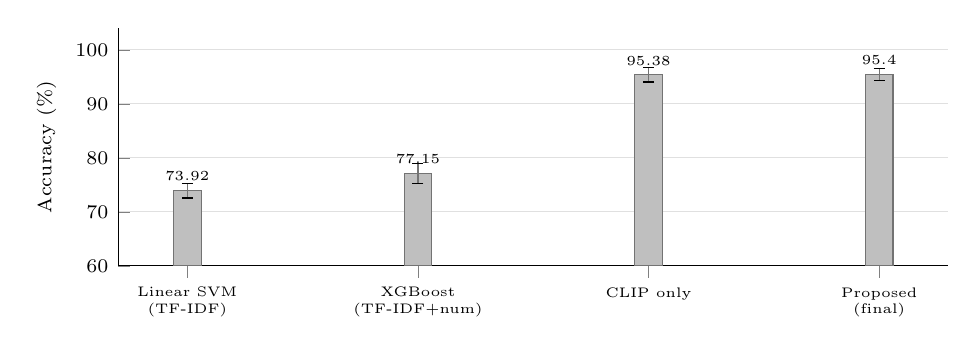
\begin{tikzpicture}
\begin{axis}[
  width=\columnwidth, height=4.6cm, font=\scriptsize,
  ybar, bar width=10pt, ymin=60, ymax=104,
  ylabel={Accuracy (\%)}, ylabel near ticks,
  xtick={0,1,2,3}, xticklabels={{Linear SVM\\(TF-IDF)},{XGBoost\\(TF-IDF+num)},{CLIP only},{Proposed\\(final)}},
  xticklabel style={font=\tiny, align=center},
  ymajorgrids, grid style={black!12}, axis lines*=left,
  nodes near coords, nodes near coords style={font=\tiny,
    /pgf/number format/fixed, /pgf/number format/precision=2},
  error bars/y dir=both, error bars/y explicit,
]
\addplot[fill=black!25, draw=black!55] table[x index=0, y index=1,
  y error index=2] {
0 73.92 1.35
1 77.15 1.86
2 95.38 1.33
3 95.40 1.09
};
\end{axis}
\end{tikzpicture}
\caption{Multimodal configuration against text-only baselines under the
identical grouped cross-validation protocol.}
\label{fig:baselines}
\end{figure}

Table~\ref{tab:baselines} and Fig.~\ref{fig:baselines} compare the multimodal
final configuration against two text-only baselines under the same protocol,
with all four metrics reported for every row. A linear SVM on TF-IDF features
reaches 73.93 $\pm$ 1.35 percent accuracy, and an XGBoost classifier on TF-IDF
plus auxiliary numeric features reaches 77.15 $\pm$ 1.86 percent---both
roughly 18--21 percentage points below any CLIP-containing configuration. This
confirms that visual features provide the primary discriminative signal for
this manipulation-detection task. We include the CLIP-only row deliberately:
it is the baseline the proposed configuration must beat, and
Section~\ref{sec:fusion} shows it does not beat it on any measure.

It is worth noting which rows moved most when duplicate-aware folds replaced
random ones. The two text-only baselines lost 2.4 and 1.8 points
(76.30 $\rightarrow$ 73.93 and 78.95 $\rightarrow$ 77.15), while every
CLIP-containing configuration moved by at most 0.35. Near-duplicate images
share a BLIP caption almost verbatim, so a text model that meets the same
caption in training and test gains far more from the leak than a visual model
does. This is a concrete argument for group-aware folds in caption-based
misinformation work generally, not only here.

\subsection{Key Observations}

\begin{itemize}
\item CLIP visual features alone match or exceed every text-inclusive
configuration on this dataset---the dataset's manipulations are photographic,
not text-embedded, so visual features dominate.

\item OCR contributes no measurable benefit on BanFakeMM specifically; this is
not generalized as a claim about Bangla misinformation broadly, since
MultiBanFakeDetect \cite{multibanfake} indicates text-in-image remains a
meaningful vector in this language more broadly.

\item The zero-shot distribution-shift gap (95.40 $\rightarrow$ 85.6 percent
accuracy, 95.70 $\rightarrow$ 73.0 percent fake-recall) is substantial even
for a well-performing same-distribution classifier.

\item Almost all of that gap is a \emph{calibration} effect: a threshold
chosen on disjoint validation data recovers accuracy to 91.8 percent and
fake-recall to 95.0 percent with no retraining at all.

\item Supervised adaptation on 300 target-style images adds nothing measurable
once the threshold is selected honestly ($+0.0$ points, 95 percent CI
$[-3.6, +3.6]$, McNemar $p = 1.00$). Where the threshold is tuned on the
evaluation set instead, the same comparison appears to show a 1.5-point gain.

\item Near-duplicate contamination is real but small here, and it hurts text
models far more than visual ones: content screening moved the text-only
baselines by up to 2.4 points and every CLIP-containing configuration by at
most 0.35. Removing the 3.0 percent of contaminated test images changed the
distribution-shift conclusions by no more than 0.4 points.
\end{itemize}

%==============================================================
\section{Discussion}
%==============================================================

\subsection{Visual-versus-Textual Modality Trade-off Analysis}

The ablation outcomes are explained by the nature of BanFakeMM's manipulations
rather than by any inherent weakness in text-based features generally. The
dataset's fake images are produced through pixel-level editing or full-image
AI generation, so the evidence of manipulation is encoded directly in visual
texture, lighting consistency, and generation artifacts---exactly the signal
CLIP's visual encoder is trained to capture. A caption or OCR-derived text
feature can only reflect manipulation indirectly, which is a much weaker and
noisier proxy; this explains both OCR's near-chance standalone performance and
CLIP's dominance once included. This also bounds the finding: on a corpus
where manipulation is carried by embedded text, the ranking could invert.

The absence of a measurable CISF contribution on top of CLIP is similarly
explainable rather than anomalous. CISF's neighbour-weighted fusion mechanism
is designed to sharpen a semantic embedding by borrowing signal from similar
items in the training corpus---a mechanism suited to text embeddings that
benefit from smoothing against semantically related neighbours. One plausible
explanation for CISF's limited effect on CLIP is that CLIP's visual embedding
already encodes a rich, high-dimensional description of the image directly
from pixels, leaving comparatively little redundant noise for neighbour-fusion
to average away---though this is inferred from the observed ablation pattern
rather than independently verified.

\subsection{Calibration Versus Representation Under Shift}

The distribution-shift results separate two failure modes that a single
accuracy figure conflates. A model can fail under shift because its learned
representation does not transfer, or because its representation transfers but
its operating point does not. Our results point firmly at the second. The
zero-shot model's ranking of shifted images by fake-probability is good enough
that a threshold of 0.08---chosen without ever seeing the test
partition---recovers 91.8 percent accuracy and 95.0 percent fake-recall.
What failed at the default 0.50 cut-off was calibration: the shifted fakes
receive systematically lower probabilities than the training-style fakes did,
so a boundary tuned for one manipulation style rejects the other.

This reframes what the 300 adaptation images were doing. Under a threshold
tuned on the evaluation set, they appeared to add 1.5 points; under a
validation-selected threshold they add nothing, because thresholding had
already captured the available headroom. Whether a larger or more diverse
adaptation set would help remains open---300 images is a small intervention
against a 1{,}600-image training set---but this experiment does not support the
claim that it does, and we do not make it.

We note the boundary of this claim: both splits come from the same benchmark
and differ in manipulation style (localized AI editing versus full-image AI
generation), not in image source or capture conditions. A shift that also
changes provenance, resolution or compression could plausibly damage the
representation itself rather than only the operating point.

\subsection{Addressing the Research Problems}

\begin{itemize}
\item \textbf{Training-data scarcity:} addressed through BanFakeMM's
adversarially constructed training set combined with an explicit, sealed
distribution-shift evaluation---rather than assuming same-distribution
accuracy generalizes to deployment.

\item \textbf{Same-distribution overstatement:} addressed by reporting the
zero-shot shifted result (85.6 percent accuracy, 73.0 percent fake-recall)
alongside the same-distribution result (95.40 percent), by selecting the
operating threshold on disjoint validation data, by screening every partition
for near-duplicates, and by retracting a previously claimed adaptation gain
that did not survive that protocol.
\end{itemize}

\subsection{Limitations and Future Directions}
\label{sec:limitations}

Several limitations bound this work, in addition to the two disclosures
already stated in Section~\ref{sec:data}.

Ground-truth labels throughout this study derive from BanFakeMM's own
deterministic construction process, so the classifier's demonstrated
competence is specific to detecting this class of algorithmic image
manipulation, not to adjudicating whether a news item's overall claim is
true. Establishing that a photograph was edited says nothing about whether the
story attached to it is accurate, and nothing in this paper should be read as
a claim about the latter.
The distribution-shift evaluation, while sealed and screened for
near-duplicates and free of threshold-selection effects, is drawn from a
second split of the same underlying benchmark; generalization to manipulation styles and image sources entirely
outside BanFakeMM, including organically collected real-world Bangladeshi
social media imagery, remains an open question.

A classifier score alone is not a verdict on a news item, and pairing this
detector with retrieval over a Bangla fact-check corpus is the obvious next
step. We do not report such a stage here because evaluating one properly
requires a labelled claim set with adjudicated verdicts, retrieval recall@$k$
against gold evidence, and an abstention analysis---none of which this paper
provides. A preliminary measurement on our own corpus suggests that step is
harder than it looks: the multilingual sentence encoder we tested does not
separate Bangla fact-check headlines well enough for reliable retrieval, since
those headlines share a fixed rhetorical template. Quantifying that, and
finding an encoder that survives it, is left to future work.

Threshold calibration is a data-centric mitigation. Architecture-level
alternatives---CLIPood's fine-tuning-based approach to CLIP
out-of-distribution generalization \cite{clipood}, domain-specific
prompt-tuning approaches such as DPOD \cite{dpod}---were not evaluated here.
Threshold-independent metrics such as AUROC and FPR@95, and calibration
metrics such as expected calibration error and Brier score, were not computed,
although the results of Section~\ref{sec:shift} suggest calibration analysis
is exactly where the remaining headroom lies. Finally, this pipeline addresses
static image manipulation; extending it to video-based misinformation would
require a substantially different technical approach.

%==============================================================
\section{Conclusion}
%==============================================================

Practical Bangla misinformation detection demands more than a
same-distribution accuracy figure---it requires a distribution-shift check
that is free of selection effects and of near-duplicate contamination, and an
honest account of what each component of the model actually contributes.

This research contributes: (1) a multimodal Bangla fake-news image classifier
combining BLIP, SBERT/CISF and CLIP features, with its final configuration
selected through per-modality ablation rather than default inclusion of every
signal; (2) an empirically justified architectural simplification---OCR
removed after ablation showed it performs near chance level; (3) a leak-free
distribution-shift protocol---content-based near-duplicate screening across
every partition, disjoint adaptation, validation and sealed test subsets, a
selection rule fixed in advance, and a single scoring of the sealed
partition---which quantifies a real zero-shot gap (95.40 $\rightarrow$
85.6 percent accuracy, 95.70 $\rightarrow$ 73.0 percent fake-recall) and shows
that a validation-selected threshold recovers it to 91.8 percent without
retraining; (4) a retracted result, reported as such: supervised adaptation on
300 target-style images adds nothing measurable once the threshold is chosen
honestly; and (5) transparent reporting of the concrete limitations of each
of these results.

The gap between a high same-distribution accuracy figure and a system that
behaves reliably outside its training distribution is real and, on this task,
substantial---but our results locate most of it in calibration rather than in
the learned representation, which is both a cheaper problem to fix and an
easier one to get wrong when the operating point is tuned on the test set.

Two directions remain open. First, this evaluation should be extended to
organically collected Bangladeshi social media imagery, where manipulation
style, provenance and capture conditions all differ from a constructed
benchmark. Second, pairing the detector with evidence retrieval over a Bangla
fact-check corpus would let it speak to the truth of a claim rather than only
the integrity of an image---but, as noted above, that requires a retrieval
component demonstrably able to discriminate between Bangla fact-check
documents, which is itself an open problem.

%==============================================================
% ACKNOWLEDGMENT -- hidden while \blindsubmissiontrue.
%==============================================================
\ifblindsubmission\else
\section*{Acknowledgment}
The authors thank [NAMES] for their support of this work. [Add funding
agency and grant number here if applicable; delete this section entirely if
neither applies.]
\fi

%==============================================================
\begin{thebibliography}{00}

% TODO(reviewer-6, BLOCKING): the BanFakeMM record could not be independently
% verified -- supply curator, year and DOI from the Mendeley Data landing page.
\bibitem{banfakemm} ``BanFakeMM: Bangla multimodal fake news dataset,''
Mendeley Data. [Online]. Available: \url{https://data.mendeley.com/}
\ifdraftnotes\\\emph{\footnotesize [DRAFT NOTE -- REMOVE BEFORE SUBMISSION]
Dataset citation incomplete: no DOI, curator name, or year could be
independently verified; the exact Mendeley record must be supplied.}\fi

\bibitem{banfakenews} M. Z. Hossain, M. A. Rahman, M. S. Islam, and S. Kar,
``BanFakeNews: A dataset for detecting fake news in Bangla,'' in
\emph{Proc. 12th Lang. Resources and Evaluation Conf. (LREC)}, Marseille,
France, 2020, pp. 2862--2871.

\bibitem{multibanfake} F. T. J. Faria \emph{et al.},
``MultiBanFakeDetect: Integrating advanced fusion techniques for multimodal
detection of Bangla fake news in under-resourced contexts,''
\emph{Int. J. Inf. Manage. Data Insights}, 2025.

\bibitem{banfakenews2} H. M. Shibu, S. Datta, M. S. Miah, N. Sami,
M. S. Chowdhury, and M. S. Islam, ``From scarcity to capability: Empowering
fake news detection in low-resource languages with LLMs,'' in
\emph{Proc. Conf. Indo NLP (IndoNLP)}, 2025, arXiv:2501.09604.

\bibitem{mmcfnd} S. Bansal, N. S. Singh, S. S. Dar, and N. Kumar,
``MMCFND: Multimodal multilingual caption-aware fake news detection for
low-resource Indic languages,'' 2024, arXiv:2410.10407.

\bibitem{eann} Y. Wang \emph{et al.}, ``EANN: Event adversarial neural
networks for multi-modal fake news detection,'' in \emph{Proc. 24th ACM
SIGKDD Int. Conf. Knowl. Discovery Data Mining}, 2018, pp. 849--857.

\bibitem{mvae} D. Khattar, J. S. Goud, M. Gupta, and V. Varma,
``MVAE: Multimodal variational autoencoder for fake news detection,'' in
\emph{Proc. World Wide Web Conf. (WWW)}, San Francisco, CA, 2019,
pp. 2915--2921.

\bibitem{spotfake} S. Singhal, R. R. Shah, T. Chakraborty, P. Kumaraguru, and
S. Satoh, ``SpotFake: A multi-modal framework for fake news detection,'' in
\emph{Proc. IEEE 5th Int. Conf. Multimedia Big Data (BigMM)}, Singapore, 2019,
pp. 39--47.

\bibitem{defame} T. Braun, M. Rothermel, M. Rohrbach, and A. Rohrbach,
``DEFAME: Dynamic evidence-based fact-checking with multimodal experts,''
2024, arXiv:2412.10510.

\bibitem{ragar} M. A. Khaliq, P. Chang, M. Ma, B. Pflugfelder, and
F. Mileti\'{c}, ``RAGAR, your falsehood radar: RAG-augmented reasoning for
political fact-checking using multimodal large language models,'' in
\emph{Proc. 7th FEVER Workshop, ACL}, 2024, arXiv:2404.12065.

% TODO(reviewer-6, BLOCKING): confirm the RAMA author list from the arXiv
% record; it could not be independently verified.
\bibitem{rama} ``RAMA: Retrieval-augmented multi-agent framework for
misinformation detection in multimodal fact-checking,'' 2025,
arXiv:2507.09174.
\ifdraftnotes\\\emph{\footnotesize [DRAFT NOTE -- REMOVE BEFORE SUBMISSION]
Author list not independently confirmed; verify against the arXiv record.}\fi

\bibitem{calm} I.-H. Hsu \emph{et al.}, ``CaLM: Contrasting large and small
language models to verify grounded generation,'' in \emph{Findings Assoc.
Comput. Linguistics: ACL 2024}, arXiv:2406.05365.

\bibitem{mmfusionnet} J. He, T. Liu, J. Zhao, and B. Turner,
``MMFusionNet: Context-aware dynamic fusion for multi-modal fake news
detection with large vision-language models,'' 2025, arXiv:2508.05684.

\bibitem{claaf} G. Mu, C. Chen, X. Li, Y. Chen, J. Dai, and J. Li,
``CLAAF: Multimodal fake information detection based on contrastive learning
and adaptive agg-modality fusion,'' \emph{PLOS ONE}, May 2025.

\bibitem{clipood} Y. Shu, X. Guo, J. Wu, X. Wang, J. Wang, and M. Long,
``CLIPood: Generalizing CLIP to out-of-distributions,'' in \emph{Proc. 40th
Int. Conf. Machine Learning (ICML)}, 2023, arXiv:2302.00864.

\bibitem{dpod} A. Bhattacharya, D. Brahma, S. Nagaje, A. Asati, V. Verma, and
S. Biswas, ``Can out-of-domain data help to learn domain-specific prompts for
multimodal misinformation detection?'' in \emph{Proc. IEEE/CVF Winter Conf.
Appl. Comput. Vis. (WACV)}, 2025, arXiv:2311.16496.

\end{thebibliography}

%==============================================================
% TRIM CANDIDATES -- to reach the ICCIT 6-page limit, remove in roughly this
% order (least damaging first):
%
%  1. CCS Concepts block -- no IEEE equivalent, pure leftover
%  2. Fig. 2 (fig2_modality_ablation)   -- Table I has the same numbers
%  3. Fig. 6 (fig6_baseline_comparison) -- Table IV has the same numbers
%  4. Sec. IV-G "Key Observations"      -- repeats IV-A / IV-D
%  5. Sec. V-C "Addressing the Research Problems" -- repeats Sec. I
%  6. Sec. I-A "Research Problems" bullets -> compress to 3 sentences
%  7. Sec. II's four "critical limitations" bullets -> one paragraph
%  8. Sec. IV-C "Final Configuration Evaluation" -> merge into IV-A
%  9. Sec. V-A paragraph 2 (CISF explanation)
% 10. Sec. IV-E confusion-matrix prose -> fold into the Fig. 5 caption
% 11. Table I rows "Caption only" and "Text only"
% 12. Fig. 1 -> swap in fig1_system_architecture_classifier_only.png and move
%     it from figure* to a single column
%
% Keep at all costs: Sec. III-B partitioning and near-duplicate screening,
% Sec. III-D threshold selection, Table II with its CI footnote, Table III
% and Sec. IV-B (the fusion answer), the retraction paragraph in Sec. IV-D,
% and the per-class metric columns. Those are the reviewer fixes.
%
% Fig. 3 (validation threshold sweep) and Fig. 5 (confusion matrices) should
% survive trimming: they are the evidence for the leak-free protocol and for
% the calibration-versus-representation argument.
%==============================================================

\end{document}
